%------------------------------------------------------------------------------
% BEGINING
%------------------------------------------------------------------------------
\documentclass{amsart}
% Packages
\usepackage[pdftex]{graphicx}
\usepackage{algorithm}
\usepackage{algorithmic}
\usepackage{amsmath}
\usepackage{epsfig}
\usepackage{changepage}
\usepackage[utf8]{inputenc}
\usepackage[english]{babel}
\usepackage{amsthm}
\usepackage{amsfonts}
\usepackage{amssymb}
\usepackage{caption}
\usepackage{enumitem}
\usepackage{multirow}
%\usepackage[
%	backend=biber,
%	style=ieee,
%]{biblatex}
\usepackage{csquotes}
\usepackage[colorlinks,linkcolor=blue]{hyperref}


\newtheorem{theorem}{Theorem}[section]
\newtheorem{lemma}[theorem]{Lemma}

\theoremstyle{definition}
\newtheorem{definition}[theorem]{Definition}
\newtheorem{example}[theorem]{Example}
\newtheorem{xca}[theorem]{Exercise}

\theoremstyle{remark}
\newtheorem{remark}[theorem]{Remark}

\numberwithin{equation}{section}

%    Absolute value notation
\newcommand{\abs}[1]{\lvert#1\rvert}

%    Blank box placeholder for figures (to avoid requiring any
%    particular graphics capabilities for printing this document).
\newcommand{\blankbox}[2]{%
  \parbox{\columnwidth}{\centering
%    Set fboxsep to 0 so that the actual size of the box will match the
%    given measurements more closely.
    \setlength{\fboxsep}{0pt}%
    \fbox{\raisebox{0pt}[#2]{\hspace{#1}}}%
  }%
}

\begin{document}
%%%%%%%%%%%%%%%%%%%%%%%%%%%%%%%%%%%%%%%%%%%%%%%%%%%%%%%%%%%%%%%%%%%%%%%%
\title{GENERAL CONSTRUCTION AND ANALYSIS OF PARALLEL MATRIX MULTIPLICATION ALGORITHMS}

%    Information for first author
\author{WENJING CUN}
%    Address of record for the research reported here
\address{Department of Applied Mathematics, Stonybrook Univ. SUNY, 
Stony Brook, New York 11790}
%    Current address
%\curraddr{Department of Mathematics and Statistics,
%Case Western Reserve University, Cleveland, Ohio 43403}
\email{wenjing.cun@stonybrook.edu}
%    \thanks will become a 1st page footnote.
\thanks{The first author was supported in part by NSF Grant \#000000.}

%    Information for second author
\author{LIHUA PEI}
\address{Department of Applied Mathematics, Stonybrook Univ. SUNY, 
Stony Brook, New York 11790}
\email{lihua.pei@stonybrook.edu}
\thanks{Support information for the second author.}

%    Information for second author
\author{YUEFAN DENG}
\address{Department of Applied Mathematics, Stonybrook Univ. SUNY, 
Stony Brook, New York 11790}
\email{yuefan.deng@stonybrook.edu}
%\thanks{Support information for the coord author.}

%    General info
%\subjclass[2000]{Primary 54C40, 14E20; Secondary 46E25, 20C20}

\date{March 29, 2018}

\keywords{Parallel Computation, Matrix Theory}
%%%%%%%%%%%%%%%%%%%%%%%%%%%%%%%%%%%%%%%%%%%%%%%%%%%%%%%%%%%%%%%%%%%%%%%%
\begin{abstract}
	This paper proposes a general vision onto the construction of the algorithms of parallel matrix multiplication in distributed-memory system. Via the analysis of the communication forest of the algorithms, this paper presents a map of the parallel algorithms for universal matrix multiplication, based on 3-dimensional hypercube algorithm with computational complexity of $O(N^3)$, and presents the experiments results of several algorithms on clusters to compare the performance.
\end{abstract}
%%%%%%%%%%%%%%%%%%%%%%%%%%%%%%%%%%%%%%%%%%%%%%%%%%%%%%%%%%%%%%%%%%%%%%%%
\maketitle
%%%%%%%%%%%%%%%%%%%%%%%%%%%%%%%%%%%%%%%%%%%%%%%%%%%%%%%%%%%%%%%%%%%%%%%%
\section{Introduction}
	High-performance algorithms of linear operations are critical for many of the computing tasks, and to promote the performance of computing in computers, the topology-based algorithms of operations on specific fields are more valuable for research, in order to promote the flexibility and robustness more regardless of the values involved.\par

	And as one of the most essential linear operations, matrix multiplication is a good start point to launch our research on abstract operation. This paper will mainly discuss about the general method of constructing algorithms for matrix multiplication, and the parallelization of it, with several classical methods as well as analysis of their performances for instance.
In this research, we have discovered a general map to organize the family of the algorithms, and with the metric of parallel efficiency of the lattice, it is now possible for mathematicians to evaluate the upper bound of the algorithms depending on any given dimensions of the matrices, 
Furtherly, this paper proposes a formulated problem to reduce the computational complexity of the algorithm of matrix multiplication, which is still not resolved, yet we will figure it as a future work to research on, to lead the way to optimize the distributed algorithms with computational complexity lower than $O(N^3)$.\par

	The organization of this paper is as the following: Section 2 will present the general idea of designing the algorithms of matrix multiplication on 3D hypercube, based the maps between sets of coordinates. In Section 3, we will propose the problem of constructing the communication forest among the computation nodes, while proceeding the parallel algorithms, and organize the family of the parallel algorithms based on 3D hypercube. Then Section 4 will present the analysis of several classical parallel algorithms for matrix multiplication and propose a general algorithm for constructing the distributed plan for universal matrix multiplication. Finally this paper will propose a problem of reducing the computational complexity, and summarize the construction of algorithms.\par
%%%%%%%%%%%%%%%%%%%%%%%%%%%%%%%%%%%%%%%%%%%%%%%%%%%%%%%%%%%%%%%%%%%%%%%%

\section{Construction of matrix multiplication in 3D hypercube}
Firstly, we shall review the naïve algorithm of matrix multiplication.\par
%% --Algorithm 2.1--%%
\begin{algorithm}[t] 
\caption{(Naive Algorithm)}
\begin{adjustwidth}{0cm}{1cm} 
\textbf{Input:} $A\in \mathbb{R}^{m\times l},B\in \mathbb{R}^{l\times n}$\\
\textbf{Output:} $C\in \mathbb{R}^{m\times n}$\\
\textbf{for} $i=1:m $\textbf{ do}\\
\end{adjustwidth}
	\begin{adjustwidth}{1cm}{1cm}
	\textbf{for} $i=1:l $\textbf{ do}\\
	\end{adjustwidth}
		\begin{adjustwidth}{2cm}{1cm}
		\textbf{for} $i=1:n $\textbf{ do}\\
		\end{adjustwidth}
			\begin{adjustwidth}{3cm}{1cm}
			$C_{ik}=C_{ik}+A_{ij}\cdot B_{jk}$\\
			\end{adjustwidth}
\begin{adjustwidth}{0cm}{1cm} 
\textbf{Return } $C$\\
\end{adjustwidth}
\end{algorithm}
%% --END Alg 2.1-- %%
Naïve algorithm is the direct definition of matrix multiplications for any given pair of matrices: $A\in R^{(m\times l)},B\in R^{(l\times n)}$, where $m,l$ and n are some positive integers. And if we just focus on one final result in $C=A\cdot B$, namely $C_{ij}$, then we have:
\begin{equation}
C_{ik}=\sum_{j=1}^{l}(A_{ij}\cdot B_{jk})
\end{equation}

Then regardless of the actual values of $A_{ij}$ and $B_{jk}$, formula (1) reveals the information that $C_{ik}$ only results from the values in the coordinates depending on three indices i,j and k, namely $(i,j,k)$. Then group all $(i,j,k)$ corresponding to the coordinates in $A$ and $B$ together, we may expect there is a well-defined map from such a set of $(i,j,k)$ to that of $(i,k)$ in $C$.\par
Sourced from such an idea, and in order to make the algorithms totally independent of the values involved, so that can be flexible and robust, we will define such a map from a set of coordinates to another one in the first subsection.\par

%% ------------ Subsection 2.1 ------------ %%
\subsection{Coordinate Set and Operation Map}
Maps between sets of values with associate coordinates are often independent of the values involved, but more like the relationship among the indices of coordinates. So to abstract such relationships, we proposed the concept called operation map, of which the definition is as the following:
\begin{definition}
An operation map is a map from one set A to another set B, where there are two injective maps $L_1:C\to A, L_2:C\to B$, and C is a set with a well-defined operation function $\tau$.
\end{definition}
For convenience, we denote such an operation map $f$ as: $f_{C,\tau}:A\to B$, and name $L_1,L_2$ as the coordinate maps. Here A and B are the topologies from which the sets of values in $C$ abstracted into, and sourcing from the most intuitive concept in geometry, we call $A$ and $B$ the corresponding coordinate sets.
And an abstract operation map has a property sourced from the abstraction of the value set to coordinate sets:\
% Theorem 2.1
\begin{theorem}
Given an operation map $f_{C,\tau}:C_1\to C_2$, if $S$ is closed under a well-defined operation $\tau$ , or say $G$ is an algebraic group, then for any subset $S\subseteq G$, $f_{C,\tau}:C_1\to C_2$ is also an operation map. Vice Versa.
\end{theorem}
Such a property shows the stability of an operation map regardless of the values when the inputs in conservative of the algebraic operation.\par
For a series of operation maps, they will follow the chain rule if they follow Theorem 2.1:
% Theorem 2.2
\begin{theorem}
Given a set $G$ that is closed under a series of operations $\tau_1,...,\tau_n$, a series of sets $C_1,...,C_n$, also a series of subsets of $G, S_1,...,S_n$, there exist at least $n$ operation maps:
\begin{equation}
(f_1)_{S_1,\tau_1},...,(f_n)_{S_n,\tau_n}
\end{equation}
And $(f_1)_{S_1,\tau_1},...,(f_n)_{S_n,\tau_n}$ is also an operation map.
\end{theorem}

Following the chain rule in the opposite direction, if an abstract operation map $f_(G,\tau):C_1\to C_2$ can be decomposed into a series of abstract operation maps, then we say $f_(G,\tau)$ is separable.\par
The third property we raise here shows one additional great value of abstract operations, that is the flexibility, aka the scalability in computational engineering, if the operation map can be conservative in topology:
% Theorem 2.3
\begin{theorem}
Given two homomorphic algebraic structures $G_1$ and $G_2$, closed under two operations $\tau_1$ and $\tau_2$ respectively, if $S_1\subseteq G_1$ and $S_2\subseteq G_2$ are two subsets, and an operation map $f_(S_1,\tau_1):C_1\to C_2$, then $f_(S_2,\tau_2):C_1\to C_2$ is also an operation map.
\end{theorem}
In the next subsection, we will present the ideas of abstracting the process of matrix multiplication, based on the naive algorithm 2.1, into a separable operation map composed by several independent stages, and shows the methodology to parallelize the algorithm.\\



%% ------------ Subsection 2.2 ------------ %%
\subsection{Algorithms Based on 3-Dimensional Hypercube}
	To abstract the naïve algorithm 2.1 into the operation maps into operations maps mentioned in the previous subsection, the first step is to split all the multiplications between a pair of scalars out, then for the 3D-hypercube algorithm, this step means an abstract operation map from a coordinate set $C_{11}$ to the other one $C_{12}$. Since the original coordinate set represents the positions of all the entries of $A$ and $B$, then we denote the set of the coordinate as:
\begin{equation}
C_A=\mathbb{Z}/{m\mathbb{Z}}\times \mathbb{Z}/{l\mathbb{Z}},
C_B=\mathbb{Z}/{l\mathbb{Z}}\times \mathbb{Z}/{n\mathbb{Z}}
\end{equation}

And define the following abstract operation map:
\begin{equation}
(f_1)_{\mathbb{R},\times}:C_A\times C_B\to C_{mult3D}
\end{equation}
where $C_{mult}=\mathbb{Z}/{m\mathbb{Z}}\times \mathbb{Z}/{l\mathbb{Z}}\times \mathbb{Z}/{n\mathbb{Z}}$, "$\times$" is the scalar multiplication and:
\begin{equation}
(f_1)_{\mathbb{R},\times}((r_a,c_a),(r_b,c_b))=
\left\{
\begin{array}{ll}  
             (r_a,c_b,c_a), &\text{if } c_a=r_b  \\ 
             \varnothing, &\text{otherwise}
\end{array}
\right.
\end{equation}
\par
	This abstract operation map represents the process: $A_{ij}\cdot B_{jk}$, and from $C_{mult}$, it can be observed that all the mapping can be described as the following figure:
% figure 3D operation map #1
\begin{figure}[h]
	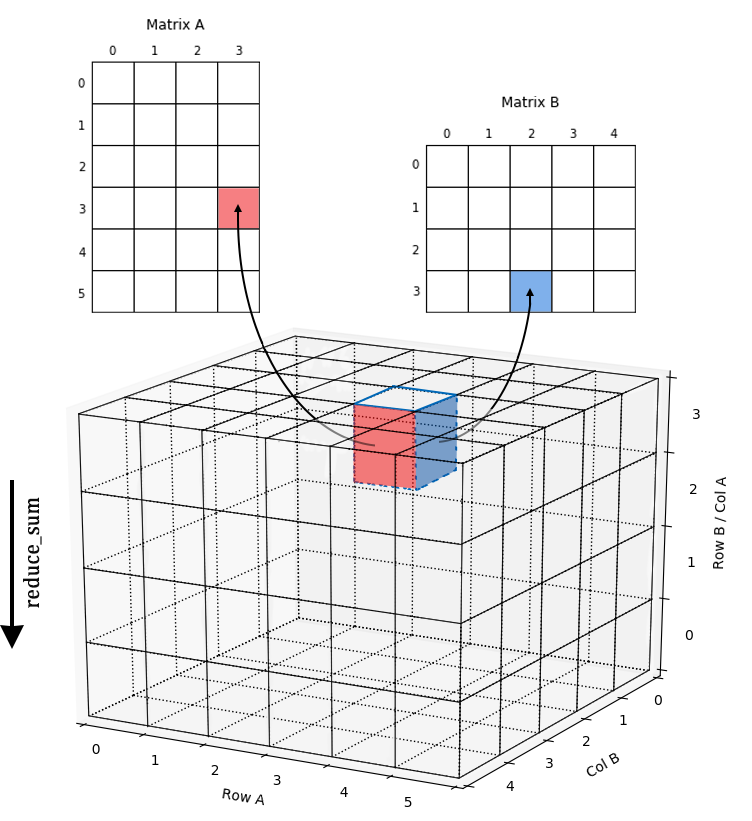
\includegraphics[scale=0.45]{Figures/Matrix3d.png}
	\caption{Operation map $(f_1)_(\mathbb{R},\times ):C_A\times C_B\to C_{\text{mult}}$}
	\label{Fig:1}
\end{figure}
~\\
~\\
\par
The next process to be considered is the addition part, here since it is known that only the scalar operation is remained, and the result is a matrix $C\in \mathbb{R}^{m\times n}$, thus we define the third coordinate set as:
\begin{equation}
C_C=\mathbb{Z}/{m\mathbb{Z}}\times \mathbb{Z}/{n\mathbb{Z}}
\end{equation}\par
And the corresponding abstract operation map is defined as:
\begin{equation}
\begin{array}{l}  
             (f_2)_{R,+}:C_{mult3D}\to C_C\\ 
             (f_2)_{R,+}((r_a,c_b,c_a))=(r_a,c_b)
\end{array}
\end{equation}
Here "+" is the scalar addition.

	Observed from formula(2.7), all the 3D “cubes” in the Figure 2.1 with the same “z-value” are reduced in to one in the “xy-plane”, which can be plotted as the following:\par
% figure 3D operation map #2
\begin{figure}[h]
	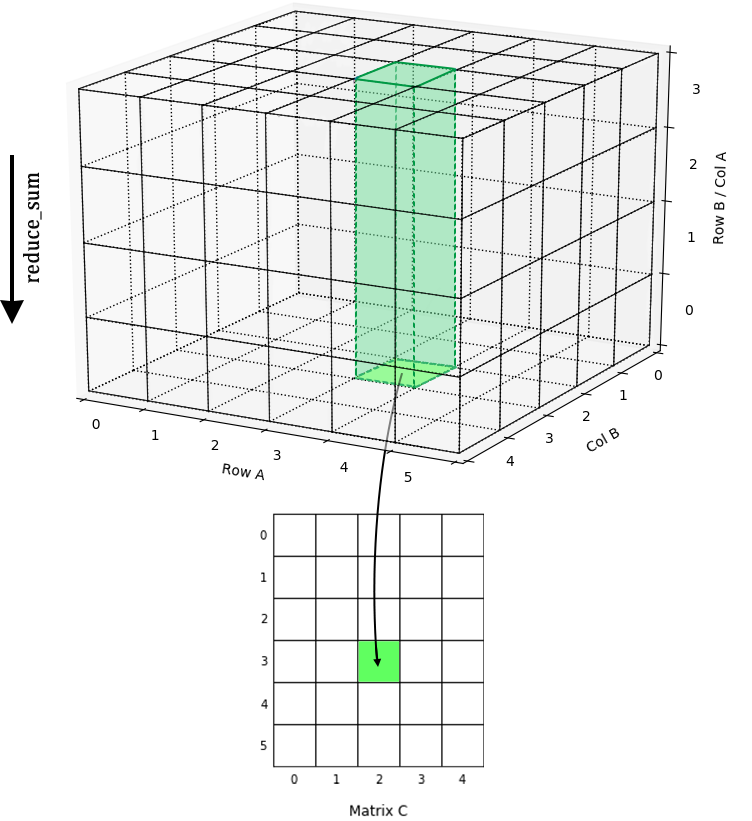
\includegraphics[scale=0.45]{Figures/Matrix3d_Reduce.png}
	\caption{Operation map $(f_2)_{F^{m\times l\times n},\text{sum}}$}
\end{figure}
~\\
\par
Now the whole process has been abstracted into a chain of abstract operation maps, for the matrix multiplication operation: $F^{m\times l}\times F^{l\times n}\to F^{m\times n}$, we can define the chain of abstract operation maps as the following:
\begin{equation}
f_{\mathbb{R}^{m\times l}\times\mathbb{R}^{l\times n},\text{matrix multiply}} = (f_1)_{\mathbb{R},\times}\circ(f_2)_{\mathbb{R},+}
\end{equation}
	where we define $f_{\mathbb{R}^{m\times l}\times\mathbb{R}^{l\times n},\text{matrix multiply}}(x)=x$, is a trivial abstract operation map directly representing that: $C=AB$.\par
	For a local-memory system, there seems nothing to modify (2.7) for such a fixed chain, but to a distributed-memory cluster, we can add one more abstract operation map to each computing node p, $g_{R,=}$, where "=" simply means the identity operation, but can filter the coordinates for each node, and we define it as:
\begin{equation}
\begin{array}{l}  
g_{\mathbb{R},=}:C_{mult3D}\to C_{mult3D}\\
g_{\mathbb{R},=}((r_a,c_b,c_a))=
	\left\{
	\begin{array}{ll}  
          (r_a,c_b,c_a), &\text{if } (r_a,c_b,c_a)\in U_p  \\ 
          \varnothing, &\text{otherwise}
	\end{array}
	\right.
\end{array}
\end{equation} 
\par
	Here $U_p$ is a custom set chosen for each node $p$, called a filtering set, represents the “blocks” chosen for node $p$ to calculate. Thus, the chain of abstract operation maps for each node $p$ is written as:
\begin{equation}
(f_p)_{\mathbb{R}^{m\times l}\times\mathbb{R}^{l\times n},\text{matrix multiply}}=
(f_1)_{mathbb{R},\times}\circ g_{mathbb{R},=}\circ(f_2)_{mathbb{R},+}
\end{equation}
This formula represents all the value-independent parallel algorithms based on Naïve Algorithm.
\par
Now we take such a case for example: if there are totally 4 nodes for computing $A\cdot B$, where $A\in \mathbb{R}^{6\times4},B\in \mathbb{R}^{4\times6}$, then choose the four filtering sets as:
\begin{equation}
\begin{array}{l}  
      U_1=\{4,5\}\times\{2,3,4\}\times(\mathbb{Z}/4\mathbb{Z}) \\ U_2=\{3\}\times\{2,3,4\}\times(\mathbb{Z}/4\mathbb{Z})\\ 
      U_3=\{3,4,5\}\times\{0,1\}\times(\mathbb{Z}/4\mathbb{Z}) \\ U_4=\{0,1,2\}\times\{0,1,2,3,4\}\times(\mathbb{Z}/4\mathbb{Z}) 
\end{array}
\end{equation}
\par
So the “blocks” in ${C_mult}$ allotted to each node are shown as the following figure:\\
% figure 3D operation map #whole
\begin{figure}[h]
	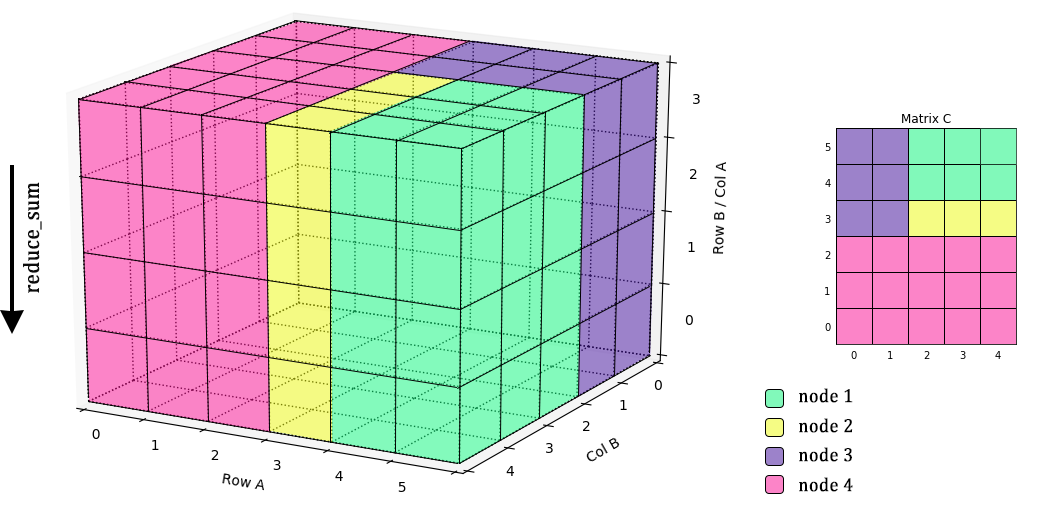
\includegraphics[scale=0.35]{Figures/Matrix3d_Filter.png}
	\caption{Parallel 3D-Hypercube}
\end{figure}
\par
	In fact, the strategy to choose filtering sets as single “cubes” that all span over z-axis, is similar to one of the popular general algorithm for parallel universal matrix multiplication, called BMR[1], if not consider the communication among the nodes. Specially, if the blocks are not finished computing at one communicating step, it can deduce many interesting algorithms, where Cannon’s algorithm[2] and SUMMA[3] are two of the famous ones.\par
	So only consider the computational part of the whole process of matrix multiplication, all the algorithms based on Naive Algorithm can be deduced by selecting the filtering sets $\{U_p\}$, so that the algorithm is presented as the following pseudocode:\par

%% --Algorithm 2.2--%%
\begin{algorithm}[h] 
\caption{(3D-Hyperblock Matrix Multiplication)}
\begin{adjustwidth}{0cm}{1cm} 
\textbf{Input:} $A\in \mathbb{R}^{m\times l},B\in \mathbb{R}^{l\times n}$\\
\textbf{Output:} $C\in \mathbb{R}^{m\times n}$\\
\textbf{if} at rank $p$\textbf{ do}\\
\end{adjustwidth}
	\begin{adjustwidth}{1cm}{1cm}
	choose $U_p=\{(i_1,j_1,k_1),(i_2,j_2,k_2),...,(i_K,j_K,k_K)\}$\\
	\textbf{for} $i,j,k$ in $U_p$ \textbf{ do}
	\end{adjustwidth}
		\begin{adjustwidth}{2cm}{1cm}
		$C_{ik}=C_{ik}+A_{ij}\cdot B_{jk}$\\
		\end{adjustwidth}
\begin{adjustwidth}{0cm}{1cm} 
\textbf{Return } $C$\\
\end{adjustwidth}
\end{algorithm}
~\\~\\~\\
\par
	The members in the 3D-Hyperblock family often have the best potential in minimizing the time in communication, however, while dealing with large-scale matrices, the buffer size often becomes a problem for the cluster to limit the total size of data to be deployed onto each computation node. Therefore, each such optimization in communication involves deploying the best subset $V_p\subseteq U_p$, and find the best communication tree to pass the data among the nodes, in order to finish the tasks undertaken by $U_p$ efficiently, which is sophisticated while dealing with such $P$ cubes simultaneously.\par

	In the next section, we will discuss the influence of limiting buffer size on designing the communication part for a parallel algorithm, and find out a general map for designing the algorithm for parallel matrix multiplication.\par


%%%%%%%%%%%%%%%%%%%%%%%%%%%%%%%%%%%%%%%%%%%%%%%%%%%%%%%%%%%%%%%%%%%%%%%%
\section{Communication in 3d-hypercube}
	Allocation of blocks of operations to each computational node is straightforward for 3D hypercube algorithms, however, while dealing with large-scale matrix multiplications, the restricted buffer size will limit the size of data stored onside each node.\par
	Generally, when a parallel program allows all the nodes to own all the necessary data already, in terms of the algorithm itself, the cost of communication can be minimized. Otherwise, one node lacking necessary data needs to fetch those needed from the other ones. So for parallel matrix multiplication, referring to algorithm 2.2, often we can only deploy part of $U_p$ onto node $p$, then following the communication tree, at each step, one need to finish as much as computation tasks with its data owing, release or send the data no longer needed, and require and receive the data needed for next step of computation.\par


%% ------------ Subsection 3.1 ------------ %%
\subsection{Communication Rules and Cost}
For convenience, we describe a “cube” assigned to node p with:\par
\begin{itemize}
\item $m_p,l_p,n_p,$ the lengths of the cube assigned to node $p$, along with x-axis, y-axis and z-axis respectively;
% figure parameters
\begin{figure}[h]
	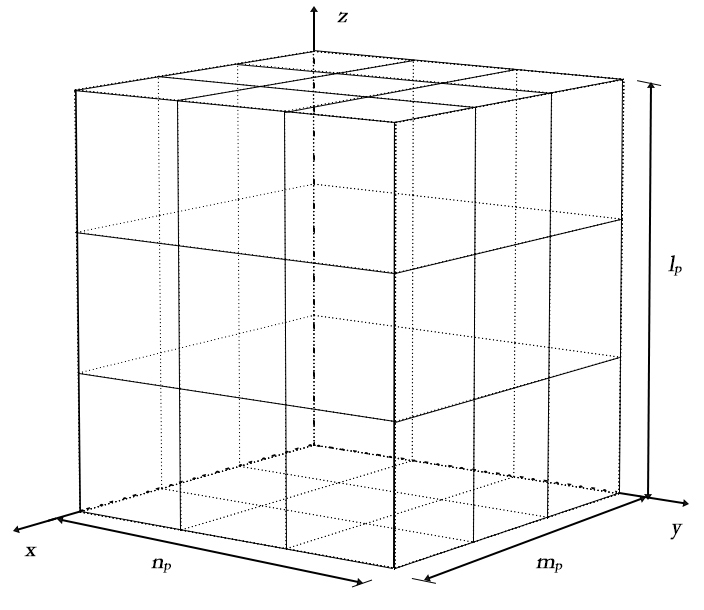
\includegraphics[scale=0.45]{Figures/cube.jpg}
	\caption{Cube Onside Node $p$}
\end{figure}
\end{itemize}

	For many of the algorithms in 3D-hypercube family, we may assume that such $P$ communication trees are similar, or out of the geometric vision, such $P$ “cubes” are similar in the following properties:\par
\begin{itemize}
\item Volume, i.e. the number of multiplication between entries;
\item Total projection area onto xz-plane and yz-plane, i.e. the total size of data needed for the computation tasks;
\item Maximum area projective onto xz-plane and yz-plane can be covered at each communication step, i.e. the maximum buffer size assigned to each core, denoted as $\text{Buffer}_p$.
\end{itemize}

The three properties above in fact determined the performance of the part of scalar (or even block) multiplication. As for the part of scalar (or even block) addition, there is only one additional property needed to be considered:\par
\begin{itemize}
\item Total projection area onto xy-plane, i.e. the size of data to be reduced onto one node.
\end{itemize}

% Rules
Then to design a smart algorithm, we may design following the rules below:\\
\textbf{Rule 3.1} The total volume of the $P$ cubes is exactly $mln$, i.e. the total volume of the whole 3D-hypercube. i.e. there would be no repetitive computational tasks among the nodes:
\begin{equation}
\sum_{p=1}^{P}m_pl_pn_p=mln
\end{equation}
\\
\textbf{Rule 3.2} The entries of two matrices can be covered by the data stored in the $P$ nodes at each communication step, so that it requires:
\begin{equation}
\sum_{p=1}^{P}\text{Buffer}_p\ge ml+ln
\end{equation}
\\
\textbf{Rule 3.3} Any entry (or block) stored onside one node can only be released if and only if all the scalar (block) multiplications involving it have been finished. So that the total cost of receiving data on node $p$ is:
\begin{equation}
T_{p,recv}=C\cdot(m_pl_p+l_pn_p-\text{Buffer}_p)
\end{equation}

\par
	From Rule 3.3, since the total number of sending is always conservative with that of receiving, so that we may estimate the average cost of communication on send-receive for each node would follow: 
\begin{equation}
\left\{
	\begin{array}{ll}  
          T_{comm,send-recv}\le\sum_{p=1}^{P}T_{p,recv}  & \text{send/require one by one}\\ 
          T_{comm,send-recv}\ge\max \limits_{p}\{T_{p,recv}\} & \text{communication parallelized}
	\end{array}
\right.
\end{equation}
\\
where the lower bound comes from the strategy that minimizing the waiting time, where we let the one with the largest demand to send nothing out.\par
	Next, based on the analysis of cost on send-recv, we are going to discuss the strategy of designing the cubes and communication tree for each node.

%% ------------ Subsection 3.2 ------------ %%
\subsection{Algorithm for Parallel Matrix Multiplication}
	In practical cases, since where all the computation nodes are in the similar conditions (in CPU, GPU, RAM, etc.), we often divide the whole 3D hypercube into $P$ similar (not necessary to be identical) cubes, and assigned with similar limits of buffer sizes.\par
	For each cube assigned to each node, due to the restriction to buffer size, our communication objective is to minimizing the time cost for communication among the nodes.\par
	So numerate $U_p=\{(x_{pi},y_{pi},z_{pi})\}$ by taking the operation map (2.9) mentioned in subsection 2.1, which is source from $A_{pk}\times B_{pk}$ at each communication step $k$, where it should satisfy that:\par
\begin{equation}
|C_{pAk}|+|C_{pBk}|\le \text{Buffer}_p
\end{equation}
\par
	So that we can see, to parallelize the matrix multiplication by adding the communication part in 3D-hypercube, the form of the operation maps can be totally conserved, and so construct a union of a series of operation maps in the same forms:
\begin{equation}
\begin{array}{ll}
&(f_{p1})_{\mathbb{R},\times}:C_{pA}\times C_{pB}\to C_{p,mult3D}\\
\Longrightarrow &
C_{p,mult3D}=\bigcup_{k=1}^{\text{total steps }K}C_{p,mult3D,k}=\bigcup_{k=1}^{K}C_{pAk}\times C_{pBk}
\end{array}
\end{equation}
Now to minimize the communication cost on each node with fixed limit of buffer size, we want to prove that:\par
\begin{theorem}
To numerate $U_p=\{(x_{pi},y_{pi},z_{pi})\}$, for $\{C_{pAk}\}$ and $\{{C_pBk}\}$ satisfying (3.5), there can exist $\{{C_{pAk}}\}$ and $\{C_{pBk}\}$ so that:
\begin{itemize}
\item For $\bigtriangleup k>1,d\in C_{pAk}\cap C_{pA,(k+\bigtriangleup k)}$ only if $d\in C_{pAk}\cap C_{pA,(k+\bigtriangleup k-1)}$.
\item For $\bigtriangleup k>1,d\in C_{pBk}\cap C_{pB,(k+\bigtriangleup k)}$ only if $d\in C_{pBk}\cap C_{pB,(k+\bigtriangleup k-1)}$.
\end{itemize}
if given that $\text{Buffer}_p\ge \min\{m_p,n_p\}$.
\end{theorem}
\par
	This theorem states the availability of Rule 3.3, so that no data (entry or block) would be sent to any one node redundantly. And the given condition can propose a general strategy for send-receive and so prove the existence.\par
	This strategy with the condition $\text{Buffer}_p\ge \min\{m_p,n_p\}$ can be stated as the following:

%% --Algorithm 3.1--%%
\begin{algorithm}[h] 
\caption{(3D-Hyperblock Algorithm with Communication)}
\begin{adjustwidth}{0cm}{0cm} 
\textbf{Input:} $A\in \mathbb{R}^{m\times l},B\in \mathbb{R}^{l\times n}$
			$,m_p,l_p,n_p,\text{Buffer}_p\in N^+,(m_p\le n_p)$\\
\textbf{Output:} $C\in \mathbb{R}^{m\times n}$\\
\textbf{if} at rank $p$\textbf{ do}
\end{adjustwidth}
	\begin{adjustwidth}{1cm}{0cm}
	$\text{Choose }U_p$
	\begin{minipage}[t]{\linewidth}
	$=\{(i_1,j_1,k_1),(i_2,j_2,k_2),...,(i_K,j_K,k_K)\} $\\
	$\subset(\mathbb{Z}_{m_p}\times\mathbb{Z}_{l_p}\times\mathbb{Z}_{n_p})\bigoplus(i_{row},j_{row},k_{row})$
	\end{minipage}

	Let $C_{pA}=(Z_(m_p)\times Z_(l_p))\bigoplus(i_low,j_low)$ and
	\par $C_{pB}=(Z_(l_p)\times Z_(n_p))\bigoplus(j_{low},k_{low})$.\\
	Sort $U_p, C_{pA}$ and $C_{pB}$ increasingly with $j$.

	Let $\text{StepSize}_A$ = $\lfloor\text{Buffer}_p/m_p\rfloor$,and initialize the buffer as:
	\begin{equation*}
		C_{pA,0}=C_{pA}[0:\text{StepSize}_A],C_{pB,0}=C_{pB}[0:\text{Buffer}_p-\text{StepSize}_A]
	\end{equation*}
	
	Set numbers of steps associated to two sets as $k_A=k_B=0$.\\
	\par
	\textbf{for }$i,j,k$ in $U_p$,
		\begin{adjustwidth}{1cm}{0cm}
		\textbf{if }$(i,j)\in C_{pA,k_A}$ and $(j,k)\in C_{pB,k_B}$ \textbf{do}
			\begin{adjustwidth}{1cm}{0cm}
			$C_{ik}=C_{ik}+A_{ij}\cdot B_{jk}$\\
			ready to send $(i,j)\in C_{pA,k_A}$ and $(j,k)\in C_{pB,k_B}$
			\end{adjustwidth}

		\textbf{else if }$(i,j)\notin C_{pA,k_A}$\textbf{do}
			\begin{adjustwidth}{1cm}{0cm}
			require $(i,j)$ from another node,\\
			pop the front of $C_{pA,k_A}$,\\
			push $(i,j)$ into the back of $C_{pA,k_A}$,\\
			$k_A=k_A+1$.
			\end{adjustwidth}

		\textbf{else if }$(j,k)\notin C_{pB,k_B}$\textbf{do}
			\begin{adjustwidth}{1cm}{0cm}
			require $(j,k)$ from another node,\\
			pop the front of $C_{pB,k_B}$,\\
			push $(j,k)$ into the back of $C_{pB,k_B}$,\\
			$k_B=k_B+1$.
			\end{adjustwidth}
		\end{adjustwidth}
	Gather the results onto the root node.
	\end{adjustwidth}

\begin{adjustwidth}{0cm}{1cm} 
\textbf{Return } $C$\\
\end{adjustwidth}
\end{algorithm}
~\\
\par
This algorithm designs a communication tree for each node, with which we can construct an algorithm with only the following two given conditions:
\begin{itemize}
\item $m_p,l_p,n_p$,i.e. a cube assigned to each node $p$;
\item $\text{Buffer}_p$.
\end{itemize}
\par
And the algorithm designed based on algorithm 3.1 is called the \textbf{Buffer Adaptive Matrix Multiplication Algorithm (BAMMA)}, which can fit to pair of matrices with random dimensions and make the best usage of buffer onside each node.\par
Next we will evaluate the performance of BAMMA, based on the variables raised in section 3.1, and show the general prediction of parallel efficiency of the algorithms for parallel matrix multiplication in 3D-Hypercube family.\par

%% ------------ Subsection 3.3 ------------ %%
\subsection{Evaluation of Performance}
To evaluate the performance, or say the total cost of time of a parallel matrix multiplication algorithm, we need to evaluate both the computational cost and the communication cost, i.e.:
\begin{equation}
T=\max \limits_{p}\{T_{p,comm}+T_{p,comp}+T_{p,idle}\} 
\end{equation}
where the $T_{p,idle}$ is the waiting time on node p.\par

	If we assigned similar cubes to $p$ nodes with similar limits of buffer sizes, then we may assume that there is a way to minimize $T_{p,idle}$ by building static routines for the whole communication forest. So that we may remove the maximum in (3.7) to estimate the total cost:
\begin{equation}
T_{total,P}\approx T_{p,comp}+T_{p,idle}
\end{equation}

	And considering the practical cases in computational clusters, we assume that the average time cost on one pair of send-receive process on one floating number (notated as $\hat{t}_{send-recv}$), and that of one arithmetical operation, (notated as $\hat{t}_{op}$), will satisfy that:
\begin{equation}
\gamma := \frac{\hat{t}_{send-recv}}{\hat{t}_{op}}
\end{equation}
and for practical cases, we assume $\tau$ is a constant value associated with particular machine, cluster topology, to be used to estimate the real fraction while running the program.\par
Now firstly, for the computational cost $T_{p,comp}$, by the operation map defined as (2.10), it sources from two parts: scalar (or block) multiplication and addition, so that we have:
\begin{equation}
T_{p,comp}=T_{p,mult}+T_{p,add}=(2\cdot m_pl_pn_p-m_pn_p)\cdot\hat{t}_{op}\approx 2m_pl_pn_p\cdot\hat{t}_{op}
\end{equation}
\par
	And for those similar $p$ cubes:
\begin{equation}
m_pl_pn_p\approx \frac{mln}{P}
\end{equation}
where P is the total number of nodes. So in total:
\begin{equation}
T_{comp}=T_{p,comp}\approx \frac{2mln}{P}\cdot\hat{t}_{op}
\end{equation}
\par
Now consider the next part of communication, it consists of two parts: send-receive in order to complete all the computations onside each cube, and the reduction with summation:
\begin{equation}
T_{comm}=T_{send-recv}+T_{reduce}
\end{equation}
\par
	For reduction, since the total cost is just the total number of entries (or blocks) need to be sent to the root node, along the z-axis, or say it is just the total projection area onto the xy-plane from the $P$ nodes. And since for each step, it involves one addition and one send/receive action, thus:
\begin{equation}
T_{send-recv}\ge C\cdot\max \limits_{p}\{m_pl_p+n_pl_p-\text{Buffer}_p\}\cdot\hat{t}_{send-recv}
\end{equation}
where generally $C$ is a constant, usually equals or larger than 2 for machines assigned with similar conditions, since one node can only do send or receive action at one single step.\par
	So in summary, we add all of the costs of parts respectively together, and it deduces the prediction formula of the total cost of time:
\begin{equation}
T_{total,P}\ge \frac{2mln}{P}\cdot\hat{t}_{op}+(\hat{t}_{send-recv}+\hat{t}_{op})\cdot
			\sum_{p=1}^{P}m_pn_p+\hat{t}_{send-recv}\cdot 2
			\cdot \max \limits_{p}\{m_pl_p+n_pl_p-\text{Buffer}_p\}
\end{equation}
\par
For the convenience to construct the space to include all the algorithms in 3D-Hypercube family, we define two new variables: \textbf{Z-variance} and \textbf{Maximum Saturabiliity}, denoted by $A_z$ and $\bar{S}$ respectively, as the following:
\begin{equation}
A_z:=\frac{\sum_{p=1}^{P}m_pn_p}{mn},
\bar{S}:=1-\max \limits{p}\{\frac{m_pl_p+n_pl_p-\text{Buffer}_p}{l(m+n)}\}
\end{equation}
here $A_z\ge 1$ and $S\in(0,1]$.\par

And by parallelizing the reducing process, the whole process to “compress” the cubes can be optimized into a flipped binary tree, so that it would take much shorter time than that in (3.13):
\begin{equation}
A_z:=\frac{\sum_{p=1}^{P}m_pn_p}{mn},
T_{reduce}=(\hat{t}_{send-recv}+\hat{t}_{op})\cdot \log_{2}A_z\cdot mn\cdot\frac{A_z}{P}
\end{equation}
with considering that the columns involving different cores can reduce parallely.\par

	And based on the assumptions of similar cubes we made above, we may deduce that:
\begin{equation}
\bar{S}:=1-\frac{\bar{m}_p\bar{l}_p+\bar{n}_p\bar{l}_p-\bar{\text{Buffer}}_p}{l(m+n)}
\end{equation}
where $\bar{m}_p,\bar{l}_p, \bar{n}_p$ and $\bar{\text{Buffer}}_p$ are set to be the similar for every node.\par

	Then consider the total cost of the matrix multiplication on a single node is always:
\begin{equation}
T_{single}=(2mln-mn)\cdot\hat{t}_{op}
\end{equation}
\par
So onside the $A_z-\bar{S}$ plane, we can now sketch the parallel efficiency:
\begin{equation}
\renewcommand\arraystretch{1.75}
\begin{array}{rl}
\tau(m,l,n,P)\le&\frac{1}{P}\cdot\frac{(2mln-mn)\cdot\hat{t}_{op}}
				 {\frac{2mln-mn}{P}\cdot\hat{t}_{op}+(\hat{t}_{send-recv}+
				  \hat{t}_{op})\cdot \log_{2}A_z\cdot mn\cdot\frac{A_z}{P}+
				  \hat{t}_{send-recv}\cdot 2\cdot l(m+n)(1-\hat{S})}\\
\approx&\frac{mln}{mln+(\frac{1+\gamma}{2}\cdot \log_{2}A_z\cdot mn\cdot\frac{A_z}+
				   P\cdot \gamma\cdot l(m+n)(1-\bar{S}))}
\end{array}
\end{equation}

because in most of the cases, $l\gg 1$ and simplify (3.18) we can finally get:
\begin{equation}
\tau(m,l,n,P)\le\frac{1}{1+\frac{1+\gamma}{2l}\cdot A_z\cdot \log_{2}A_z+P\cdot \gamma\cdot(\frac{1}{m}+\frac{1}{n})(1-\hat{S})}
\end{equation}

\par
Here to normalize the space, we set $\hat{A}_z=1-\frac{\log_{2}A_z}{\log_{2}P}=1-\log_{P}A_z\in(0,1]$, since each node can at most own projection area mn onto xy-plane, and for any one column along the z-axis, there are at most P segments belong to different nodes. So that:
\begin{equation}
\tau(m,l,n,P)\le\frac{1}{1+\frac{1+\gamma}{2l}\cdot \log_{2}P\cdot P^{1-\hat{A}_z}\cdot(1-\hat{A}_z)
			+ P\cdot \gamma\cdot(\frac{1}{m}+\frac{1}{n})(1-\hat{S})}
\end{equation}
\par
Now with formula (3.22), we can easily predict the upper bound of the parallel efficiency by given certain $m,l,n,P,\hat{m}_p,\hat{l}_p,\hat{n}_p$ and $\\hat{text{Buffer}}_p$, and we can also locate the algorithms inside the space, with the metric of parallel efficiency.\par

%% ------------ Subsection 3.4 ------------ %%
\subsection{3D-Hypercube Family}
Out of vision of the algorithm designer, it cannot be directly indicated from formula (3.22) that how to choose $\{m_p,l_p,n_p\}$ for given $m,l,n$ and $\text{Buffer}_p$, but with which we may estimate the performance of a parallel algorithm for matrices with certain dimensions, and so support us to promote the algorithm.\par
For classical method, such as Cannon’s method[2], Fox method[1], and SUMMA[3], they all focus on dividing the hypercube into cubes with special shapes following some certain rules, as shown in the following figure for example:
% Figure: Classical Methods
\begin{figure}[h]
	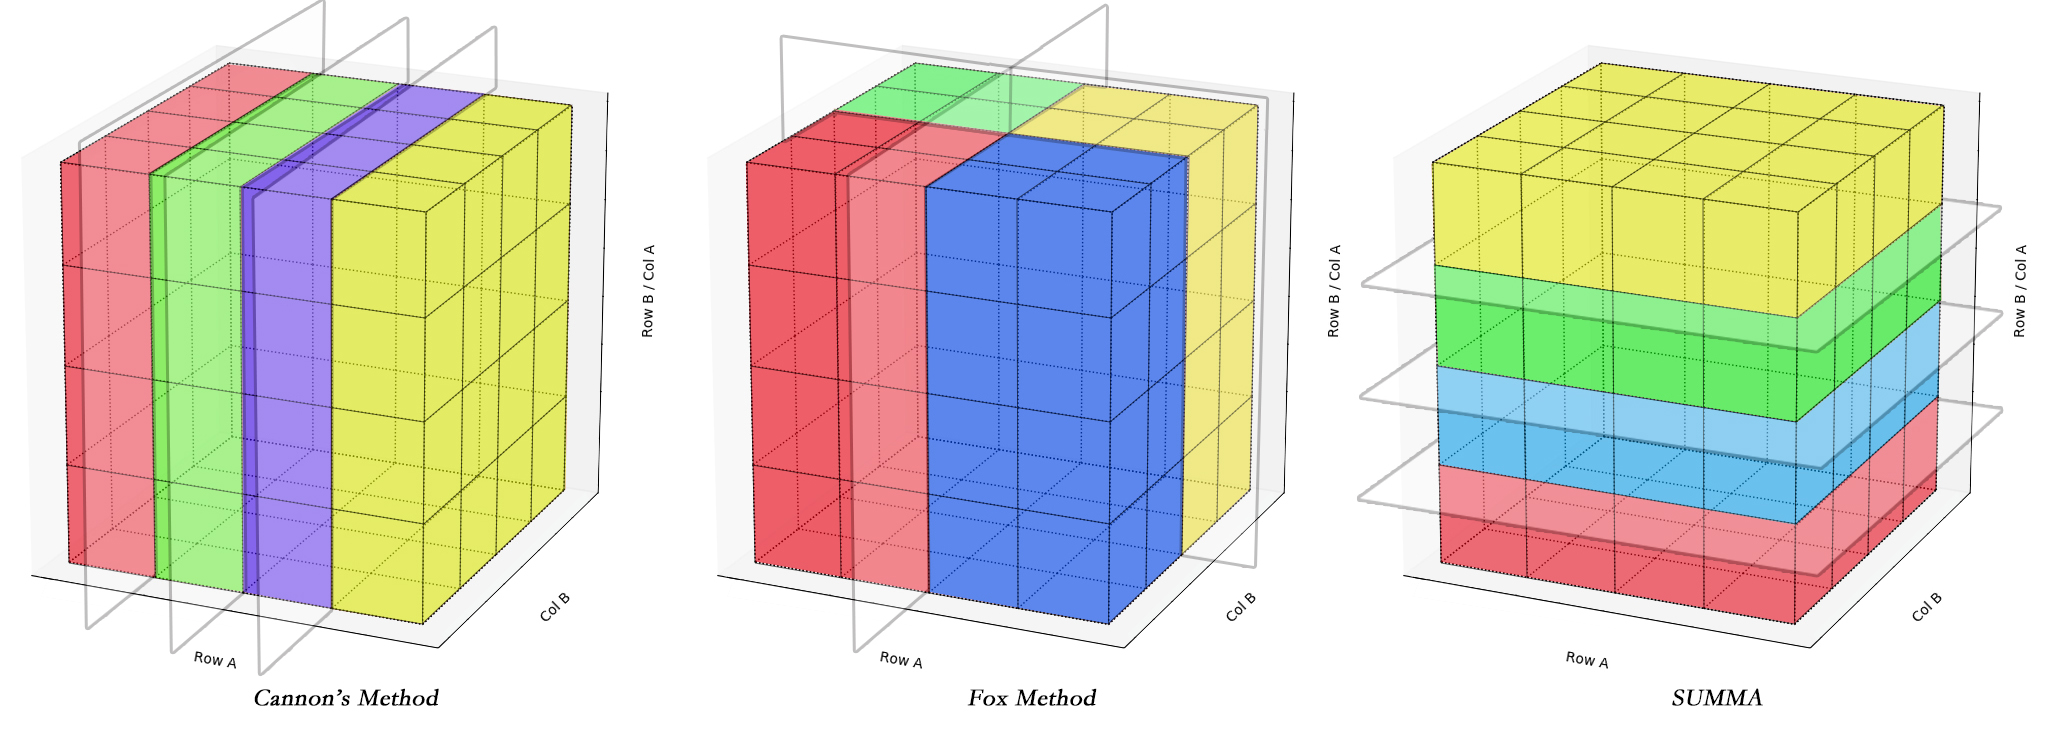
\includegraphics[scale=0.18]{Figures/3DAlg.jpg}
	\caption{Some Classical Methods}
\end{figure}
\par
	But due to different dimensions of matrices involved in the multiplication, one certain strategy to design the shape of cubes can comparatively result in different performances. Here we may plot three different color maps to show the distributions of 3D-Hypercube algorithms for parallel matrix multiplication, with the metric of parallel efficiency $\tau_{no gather}(m,l,n,P)$ defined in (3.22), under 3 different sets of dimensions, namely $m,l$ and $n$:
% Figures Performances
\begin{figure}[h]
	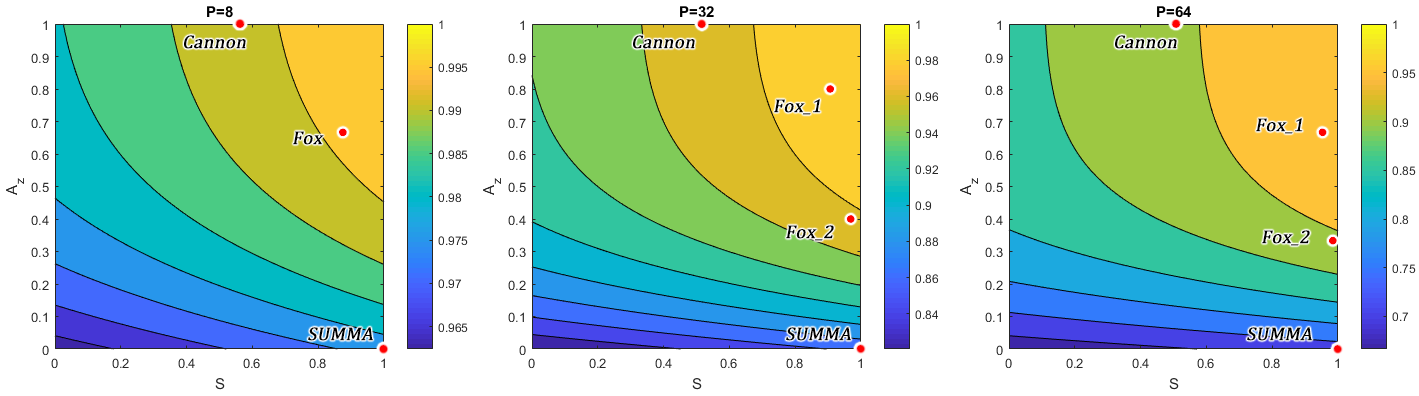
\includegraphics[scale=0.32]{Figures/Regular.png}
	\caption{Efficiency Distribution: Square Matrices $_{(m=l=n=1024,\tau=1)}$}
\end{figure}
\begin{figure}[h]
	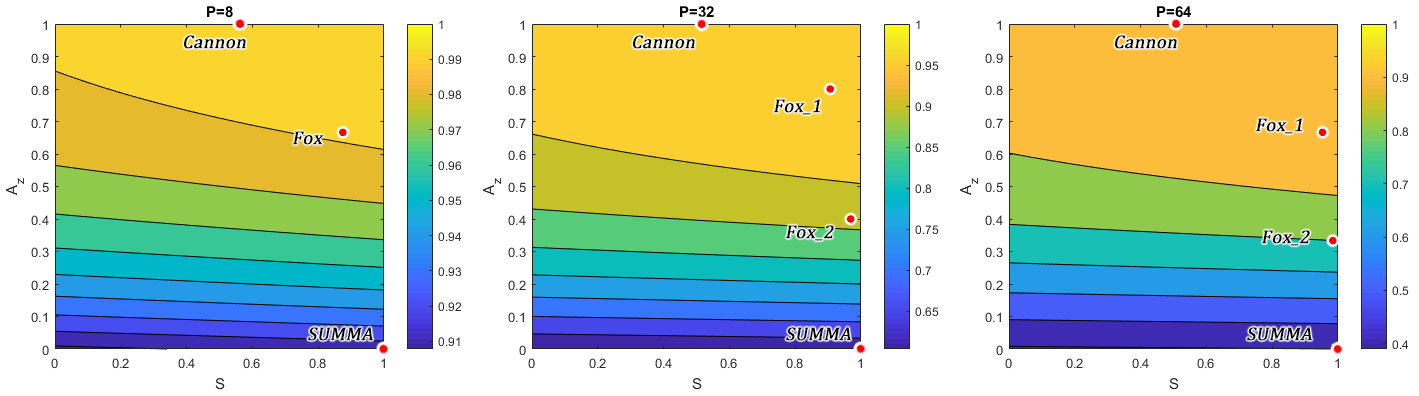
\includegraphics[scale=0.32]{Figures/Tall.png}
	\caption{Efficiency Distribution: Tall Matrices $_{(m=n=512,l=4096,\tau=1)}$}
\end{figure}
\begin{figure}[h]
	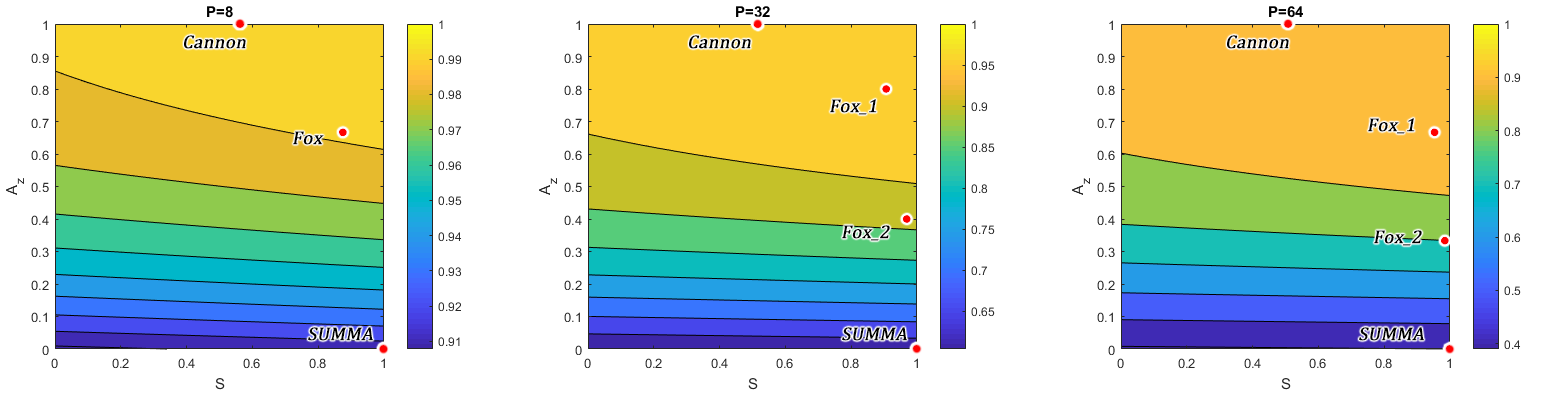
\includegraphics[scale=0.32]{Figures/Flat.png}
	\caption{Efficiency Distribution: Flat Matrices $_{(m=n=2048,l=256,\tau=1)}$}
\end{figure}
\par
So from the colormaps above, we may conclude some general ideas for constructing the algorithms for parallel matrix multiplication based on 3D-Hypercube:
\begin{itemize}
\item It would be hard to increase $\hat{A}_z$ and $\hat{S}$ with limited buffer size;
\item When $l$ is larger than $m$ and $n$, it would be better to be prior to slice the whole hypercube along z-axis, which means smaller $\hat{S}$ can compromise to smaller $\hat{A}_z$;
\item When $l$ is smaller than $m$ and $n$, it would be better to let each cube cover more blocks along the z-axis;\
\end{itemize}
\par
And we have also raised some observations from the defined variables up to now:
\begin{itemize}
\item If a cube on node $P$ is more regular, i.e. $m_p,l_p$ and $n_p$ are closer to each other, then with fixed volume $m_pl_pn_p, m_pl_p+n_pl_p$ can be smaller so that it can be more possible to increase $\hat{S}$;
\item The larger the limit of buffer size $\text{Buffer}_p$ is, the more that both $\hat{A}_z$ and $\hat{S}$ can increase;
\item For matrices with larger scale, the proportion of computations would be larger, so that the distribution of such colormap would be closer to 1.
\end{itemize}
\par
Based on those strategies, though we cannot reduce the total cost of computation, we can estimate and help to search out the best 3D-Hypercube algorithm for parallel matrix multiplication, adaptive to certain matrices dimensions, limited buffer size and some other specific conditions.\par


%%%%%%%%%%%%%%%%%%%%%%%%%%%%%%%%%%%%%%%%%%%%%%%%%%%%%%%%%%%%%%%%%%%%%%%%
\section{Application of 3d-hypercube algorithm}
	In this section, we designed a series of experiments to verify our estimations of parallel efficiency using formula (3.22).\par
	From formula (3.22), we want to find out the relationship between the parallel efficiency of a constructed 3D-hypercube algorithm and a few variables, namely the dimensions of matrices, buffer size, and the number of nodes.\par
	We designed the experiments consist of two parts: one for \textbf{estimating $\tau$} and the other one for \textbf{measuring time cost for particular algorithms}, all the experiments were tested in the SeaWulf Clusters%
%%%%%%%%%%%%%%%%%%%%%%%%%%%%%%%%%%%%%%%%%%%%%%%%%%%%%%%%%%%%%%%%%%%%%%%%
\footnote{Seawulf Clusters: \url{https://it.stonybrook.edu/help/kb/understanding-seawulf}}%
%%%%%%%%%%%%%%%%%%%%%%%%%%%%%%%%%%%%%%%%%%%%%%%%%%%%%%%%%%%%%%%%%%%%%%%%
, and run with the same one testing program, which is developed with MPI for C/C++ and is capable of parallel communication, and parallel matrix multiplication of complexity $O(N^3)$.\par

\subsection{Estimating the Value of \textbf{$\tau$}}
	As mentioned in Subsection 3.3 and referring to definition (18), $\tau$ is presumed as a constant value, associated with particular clusters with P cores. We ran the testing program to test two jobs: one for multiplying two matrices, both of dimensions $1024\times 1024$, and the other ones for broadcasting an $1024\times 1024$ matrix from each of $P$ cores one by one, so that to measuring the average costs, on unit send-receive communication, and floating operation.\par
	For taking the average, we have run two jobs both for 10 times, in 8, 32 and 64 cores assigned by SeaWulf
respectively. And the results are shown as below:\par

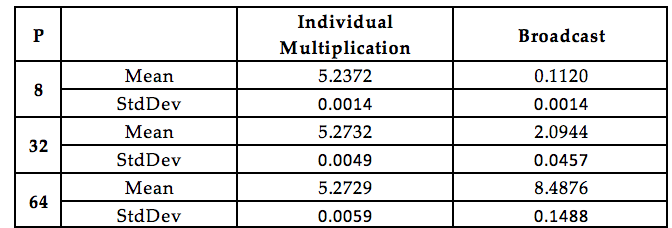
\includegraphics[scale=1]{figures/table_1.png}

So with these data, we can calculate $\gamma$ respective to each $P$ following the deduction below:

\begin{equation}
	\frac{T_{becast}}{T_{mult}} = \frac{P(P-1)\cdot 1024^{2} \cdot \hat{t}_{sendrecv}}{(C_{program} \cdot 1024^3 - 1024^2) \cdot \hat{t}_{op} } = \frac{P(P-1)}{C_{program} \cdot 1024 -1} \cdot \gamma
\end{equation}

Here $C_program$ means the account of floating operations executed per step in a practical program for matrix multiplication. However, in practical cases, it is tough to measure $C_program$ stably and precisely, so compromising to experimental cases, formula (31) is modified as the following:

\begin{equation} 
	%need to fix how to add  mark down note
	\renewcommand\arraystretch{1.75}
	\begin{array}{rl}
	\tau(m,l,n,P) =& \frac{1}{P} \cdot \frac{mln \cdot T_{mult \_ per \_ step}}{\frac{mln}{P} \cdot T_{mult \_ per \_ step} + (\hat{t}_{send-recv} + \hat{t}_{op}) \cdot \log_{2} A_{z} \cdot mn \cdot \frac{A_{z}}{P} + \hat{t}_{sendrecv} \cdot 2 \cdot l}\\ 
	=& \frac{1}{1 + \frac{\hat{t}_{sendrecv} + \hat{t}_{op}}{T_{mult \_ per \_ step} } \cdot \frac{\log_{2} \hat{A}_{z}}{l} \cdot \hat{A}_{z} + \frac{2 \cdot \hat{t}_send-recv}{T_{mult \_ per \_ step}} \cdot P \cdot (\frac{1}{m} + \frac{1}{n})(1- \bar{S}) }
	\end{array}
\end{equation}

Here $T_{mult \_ per \_ step}$ is the time cost per step in the loop of a matrix multiplication in programming.
		
		Then comparing to formula (32), it is reasonable to obtain the following relationship:

\begin{equation}
\gamma \approx \frac{2 \cdot \hat{t}_{sendrecv}}{T_{mult_per_step}} = 2 \cdot \frac{T_{bcast} / P(P-1) \cdot 1024^2}{T_{mult}/(1024^3)} = \frac{2048}{P(P-1)} \cdot \frac{T_{bcast}}{T_{mult}}
\end{equation}

So the estimated value of each $\gamma$ is calculated as the following:

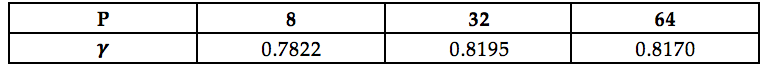
\includegraphics[scale=1]{figures/table_2.png}

It has to be admitted that there values are less than the real ones due to those not considered, and the communication performance is usually more complicated in parallel program, than that analyzed in theory so that hard to obtain the correct $\gamma$.

\subsection{Experiments of Particular Algorithms}

For each cases with 8, 32 and 64 cores respectively, we designed 7, 10 and 10 different strategies to split the 3D hypercube and allocate the buffers in different way, so that constructed various algorithms for testing the performances of each. 

To evaluate the performance, the formula for calculating the parallel efficiency is applied here:

\begin{equation}
\tau = \frac{1}{P} \cdot \frac{T_{one \_ core}}{T_{P \_ Cores}}
\end{equation}

The plans with results  are shown as the following subsections:

\emph{4.3.1 P = 8} (total 7 cases)

(1) Cube Dimension $(m_p , l_p, n_p)$ = (128, 1024, 1024), $\bar{A_z}$ = 1:

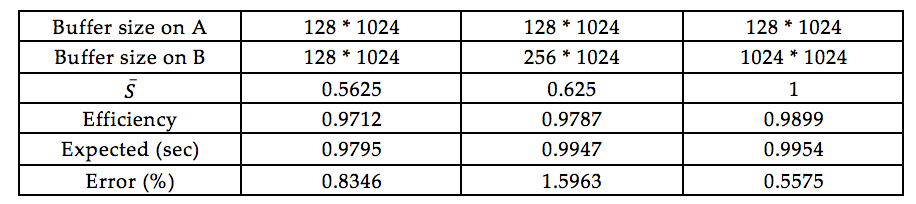
\includegraphics[scale=0.8]{figures/table_p8_1.png}

(2) Cube Dimension $(m_p , l_p, n_p)$ = (512, 512, 512), $\bar{A_z}$ = 0.6667:

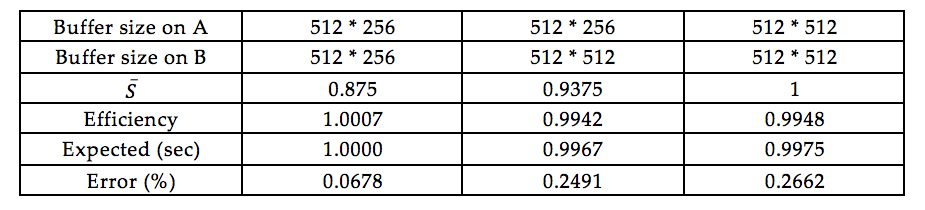
\includegraphics[scale=0.8]{figures/table_p8_2.png}

(3) Cube Dimension $(m_p , l_p, n_p)$ = (1024, 128, 1024), $\bar{A_z}$ = 0:

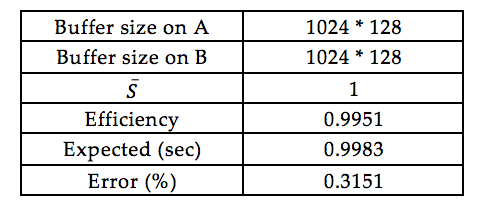
\includegraphics[scale=0.8]{figures/table_p8_3.png}

\emph{4.3.2 P = 32} (total 10 cases)

(1) Cube Dimension $(m_p , l_p, n_p)$ = (32, 1024, 1024), $\bar{A_z}$ = 1:

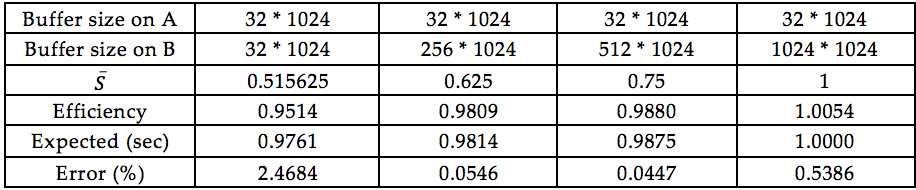
\includegraphics[scale=0.8]{figures/table_p32_1.png}

(2) Cube Dimension $(m_p , l_p, n_p)$ = (256, 512, 256), $\bar{A_z}$ = 0.8:

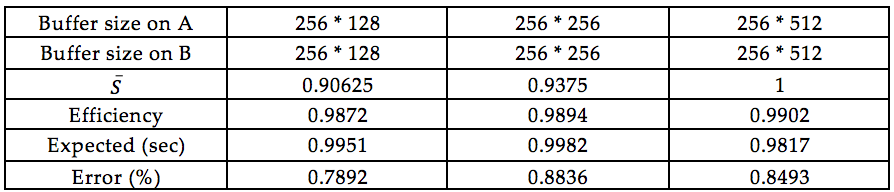
\includegraphics[scale=0.8]{figures/table_p32_2.png}

(3) Cube Dimension $(m_p , l_p, n_p)$ = (512, 128, 512), $\bar{A_z}$ = 0.4:

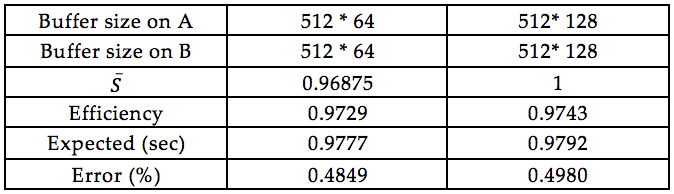
\includegraphics[scale=0.8]{figures/table_p32_3.png}

(4) Cube Dimension $(m_p , l_p, n_p)$ = (1024, 32, 1024), $\bar{A_z}$ = 0:

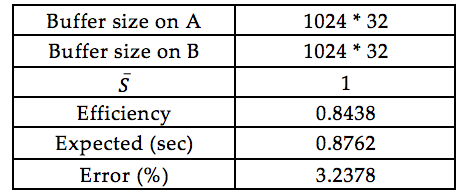
\includegraphics[scale=0.8]{figures/table_p32_4.png}



\emph{4.3.2 P = 64} (total 10 cases)

(1) Cube Dimension $(m_p , l_p, n_p)$ = (32, 1024, 1024), $\bar{A_z}$ = 1:

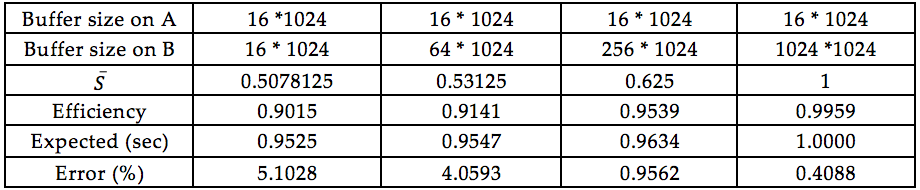
\includegraphics[scale=0.8]{figures/table_p64_1.png}

(2) Cube Dimension $(m_p , l_p, n_p)$ = (256, 512, 256), $\bar{A_z}$ = 0.6667:

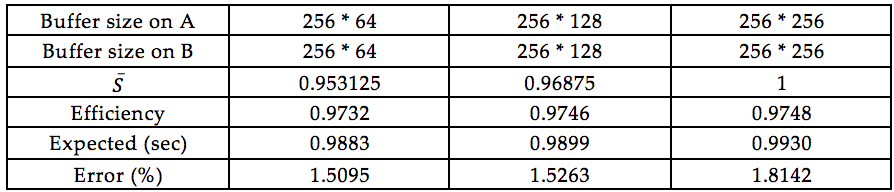
\includegraphics[scale=0.8]{figures/table_p64_2.png}

(3) Cube Dimension $(m_p , l_p, n_p)$ = (512, 128, 512), $\bar{A_z}$ = 0.3333:

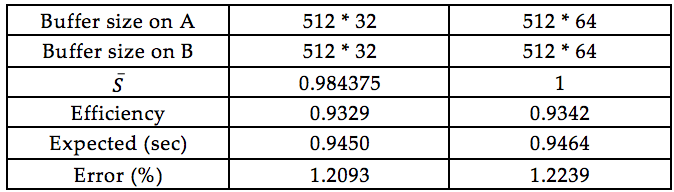
\includegraphics[scale=0.8]{figures/table_p64_3.png}

(4) Cube Dimension $(m_p , l_p, n_p)$ = (1024, 32, 1024), $\bar{A_z}$ = 0:

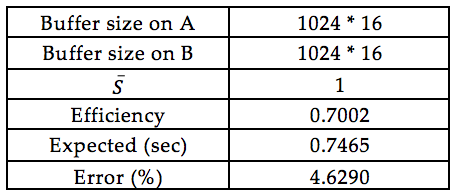
\includegraphics[scale=0.8]{figures/table_p64_4.png}

Therefore, finally we can plot the experimental results inside a 3D space together with the expected surfaces sketched from formula (32), which is shown as the following:

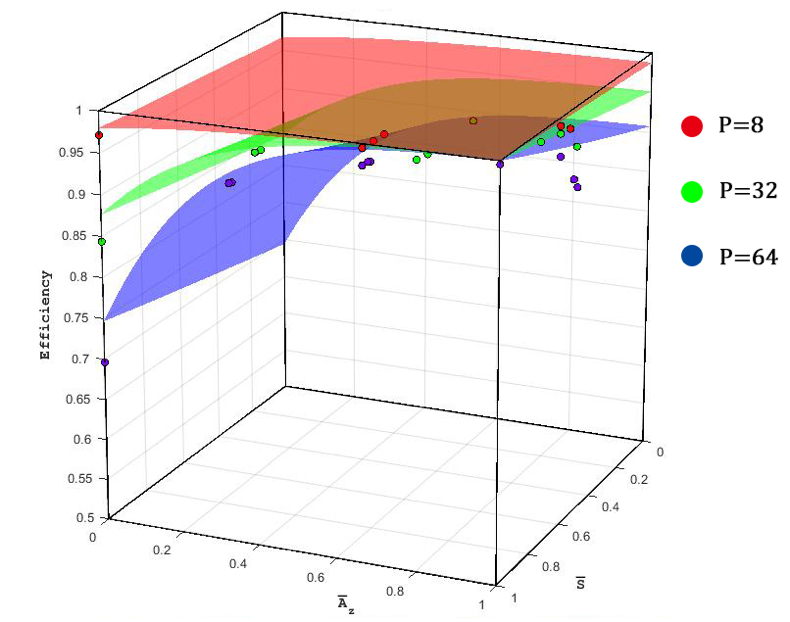
\includegraphics[scale=0.8]{figures/Efficieny.png}

Comparing to the analytic surfaces, we found that the communication parts of the algorithms are indeed affected by more other elements not discussed in this paper, which to be searched out is part of the future work on BAMMA.
%%%%%%%%%%%%%%%%%%%%%%%%%%%%%%%%%%%%%%%%%%%%%%%%%%%%%%%%%%%%%%%%%%%%%%%%
\section{Conclusions and future work}
	In this paper, we have discussed about the construction of algorithms for parallel matrix multiplication, based on 3D-Hypercube so that with total computational complexity $O(N^3)$. We have observed that the construction of such algorithm is influenced by the number of computational nodes, the dimensions of matrices and the limit of the buffer size. Concluded from both the theoretical analysis and the experiments, it is learnt that often it is better to construct the parallel algorithms considering adaptive to certain cases, described by the three variables mentioned above, rather than primly follow the rules defined by classical methods.
	
	All of the theoretical analysis is based on the assumption that all the cubes and communication trees onside the P nodes are designed similarly. So as another part of our future work on parallel matrix multiplication, we are going to dig out the possibility to design and evaluate the algorithm, with more flexibility on each specific node with specific condition respectively, so that it can adapt to more practical cases with the best performance. As one of the most latest coming work, we are going to optimize the algorithms on clusters with particular or even special topologies, using the ideas raised in this paper.
	
	And as mentioned in Section 3.2, another one of our research plans in the future is to optimize and finish the program of BAMMA, so that it can satisfy the requirement for parallel universal matrix multiplication adaptive to specific conditions, expected with better performance comparable to the classical method. And referring to a popular branch of algorithms of parallel matrix multiplication, the recursive algorithms, for instance CARMA[4] raised by the team led by James Demmel in 2013, we may need to furtherly research on the influence of sequential recursion, on the performance of a parallel algorithm of parallel matrix multiplication.
	
	Finally, as the final target to optimize the algorithm for general matrix multiplications, our group has proposed a formulated problem in 4D Hypercube, with the concepts of operation map mentioned in Section 2.1, to reduce the computational complexity of matrix multiplication, of which is lower than $O(N^3)$, inspired by the ideas[5], raised by Strassen in 1969, as well as Coppersmith and Winograd[6] in 1987. Our next target is to find a general strategy to solve to problem so that find the limit of recursive algorithms to reduce the total complexity of matrix multiplications, and furtherly construct stable and scalable parallel algorithm for universal matrix multiplication, with lower computational complexity.

\end{document}

%------------------------------------------------------------------------------
% END
%------------------------------------------------------------------------------
